\chapter{QR-Zerlegung}

\section{Definition}
Eine Matrix $A \in \mathbb{R}^{m \times n}$ , $m \ge n$ besitzt eine eindeutige QR-Zerlegung
\begin{align}
A = QR
\end{align}
mit einer orthogonalen Matrix $ Q \in \mathbb{R}^{m \times m} $ und einer oberen Dreiecksmatrix $ R \in \mathbb{R}^{n \times n}$ \cite{num1}.

Eine QR Zerlegung kann mit einer Householder-Transformation berechnet werden.

\subsection{Beispiel}
Lösung eines Minimierungsproblems
\begin{align}
\min_{x \in \mathbb{R}^n} \|Ax-b\|^2 \label{eq1}
\end{align}
mit Matrix $A \in \mathbb{R}^{m\times n}$ mit $rang(A) = n < m$ für die eine QR Zerlegung existiert.
$R$ besitzt die Gestalt 
\begin{align*}
R=	
\left(\begin{array}{ccc}
*&*&* \\ 
&*&* \\ 
& &* \\ \hline
& 0 &
\end{array} \right)
=
\left(\begin{array}{c}
\\ 
\hat{R} \\ 
\\ \hline
0
\end{array} \right) 
\end{align*}

$\hat{R}$ stellt eine obere Dreiecksmatrix dar.
Damit kann man das Minimierungsproblem wie folgt mit $A=QR$ modifizieren
\begin{align}
\min_{x \in \mathbb{R}^n} \|Ax-b\|^2 =
\min_{x \in \mathbb{R}^n} \|Q^T(Ax-b)\|^2 =
\min_{x \in \mathbb{R}^n} \|Rx-Q^Tb\|^2
\end{align}
Also löst
\begin{align}
Rx=Q^Tb \label{solvminqr}
\end{align}
das Minimierungsproblem (\ref{eq1}). Da $R$ eine Dreiecksmatrix ist, lässt sich (\ref{solvminqr}) leicht mit Rückwärtseinsetzen  lösen.

\section{Householder-Transformation}
%Ein Vektor  $v \in \mathbb{R}^n$ dann wird die $n \times n$ Matrix 
Eine Matrix $H \in \mathbb{R}^{n \times n}$ 
\begin{align}
H = I - 2 \dfrac{vv^T}{v^Tv} \label{eq:HHM}
\end{align}
wird als Householder-Transformation und der Vektor $v \in \mathbb{R}^n$ als Householder-Vektor bezeichnet.
Eine Householder-Transformation $H = I - 2 \dfrac{vv^T}{v^Tv}$ ist orthogonal und symmetrisch \cite{num1}.\\
Die Householder-Transformation spiegelt den Vektor $x$ auf die Achse $x_1$.
Dazu multipliziert man $H$ von links auf $x$
\begin{align}
Hx=\alpha e_1 \label{eq:spiegelung}
\end{align}
mit dem Skalar $\alpha \in \mathbb{R}$ und $e_1$ als ersten kanonischen Einheitsvektor. Der Householder-Vektor steht senkrecht auf der Ebene an welcher $x$ gespiegelt wird.\\
Die Abbildung \ref{fig:HHolder} veranschaulicht die Spiegelung des Vektors $x$ an der gestrichelt eingezeichneten Ebene auf die Achse $x_1$.
\begin{figure}[H]
	\centering
	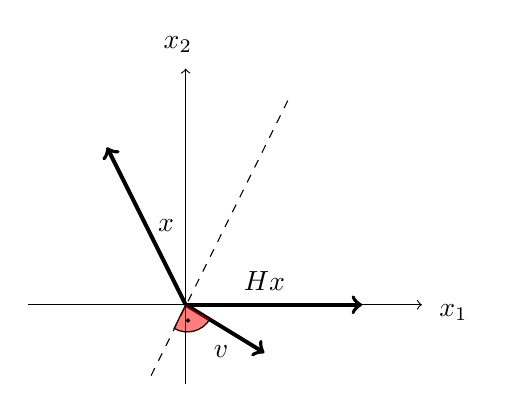
\begin{tikzpicture}

\draw[->] (-2,0) -- (3,0);
\draw[->] (0,-1) -- (0,3);

\draw[->,line width=0.5mm] (0,0) -- (-1,2);
\draw[->,line width=0.5mm] (0,0) -- (2.24,0);

\draw[dashed] (-0.44,-0.9) -- (1.34,2.68);
%\draw[->,line width=0.5mm] (0,0) -- (-0.9, 0.44);
%\draw[->,line width=0.5mm] (0,0) -- (-1,0.61);
\draw[->,line width=0.5mm] (0,0) -- (1,-0.61);





\filldraw[red, opacity=0.5] (0,0)--(-0.1467,-0.3000) arc (240:330:.3339) -- (0,0) ;
\draw[black, opacity=1] (0,0)--(-0.1467,-0.3000) arc (240:330:.3339) -- (0,0) ;
\filldraw(0.03,-0.2) circle (.02cm) ;

%Beschriftung
\draw (3.4,-0.1) node {$x_1$};
\draw (-0.1,3.3) node {$x_2$};

\draw (.45, -.6) node {$v$};
\draw (-.25, 1) node {$x$};
\draw (1,0.3) node {$Hx$};


\end{tikzpicture}
	\caption{Beispiel Householder-Transformation mit $x=(-1,2)^T$}
	\label{fig:HHolder}
\end{figure}




\subsection{Householder Vector}
Damit (\ref{eq:spiegelung}) gilt, wird der Vektor berechnet, 
indem man (\ref{eq:HHM}) in (\ref{eq:spiegelung}) einsetzt
\begin{align*}
Hx &= x - 2\dfrac{vv^T}{v^Tv} x = x - \underbrace{2\dfrac{v^Tx}{v^Tv}}_{\lambda} v = x - \lambda v \overset{!}{=} \alpha e_1 \\
&\Longrightarrow v \in \text{span}\{x - \alpha e_1\}
\end{align*}
Dadurch erhält man, dass $v$ in dem Span $x  - \alpha e_1$ liegt.\cite{num1}
%Mit $Hx = x - 2\dfrac{vv^T}{v^Tv} x = x - \lambda v \overset{!}{=} \alpha e_1$ folgt $v \in \text{span}\{x - \alpha e_1\}$. \cite{num1}\\

Setzt man $v = t(x - \alpha e_1)$ in $Hx = \alpha e_1 $(\ref{eq:spiegelung}) ein, dann erhält man 
\begin{align*}
Hx =& x - \dfrac{2}{v^Tv}v(v^Tx) = x - 2\dfrac{v^Tx}{v^Tv}v\\
=& x - 2\dfrac{ t(x - \alpha e_1)^Tx}{ t(x - \alpha e_1)^T t(x - \alpha e_1)} t(x - \alpha e_1)
= x - 2\dfrac{ (x - \alpha e_1)^Tx}{ (x - \alpha e_1)^T (x - \alpha e_1)} (x - \alpha e_1)
\\
=& x - \dfrac{(x - \alpha e_1)^Tx}{\|x - \alpha e_1\|_2^2} (x - \alpha e_1)
=\underbrace{\left(1 - \dfrac{2(x - \alpha e_1)^Tx}{\|x - \alpha e_1\|_2^2}\right)}_{ \overset{!}{=} 0 } x + \alpha e_1 \underbrace{\dfrac{2(x - \alpha e_1)^Tx}{\|x - \alpha e_1\|_2^2} }_{\overset{!}{=} 1} \overset{!}{=} \alpha e_1
\end{align*}

Damit das Letzte $=$ gilt muss gelten.
\begin{align*}
	1 &= \dfrac{2(x - \alpha e_1)^Tx}{\|x - \alpha e_1\|^2}\\
	\Leftrightarrow (x - \alpha e_1)^T(x - \alpha e_1) &= 2 x^T x - 2\alpha x_1 \\
	\Leftrightarrow x^Tx -2\alpha x_1 + \alpha^2 &= 2 x^T x - 2\alpha x_1\\
	\Leftrightarrow \alpha &= \pm \sqrt{x^Tx}
\end{align*}

Das Vorzeichen von  $\alpha = \pm \sqrt{x^Tx}$ kann man frei wählen, um $ v = x - \alpha e_1$ zu berechnen.

Wählt man das Vorzeichen positiv, kann Auslöschung auftreten, falls $x$ annähernd ein positives Vielfaches von $e_1$ ist.

LAPACK \cite{DGEQR2} vermeidet die Auslöschung, indem das Vorzeichen entgegengesetzt gewählt wird. Das bedeutet $x$ wird immer auf die gegenüberliegende Seite gespiegelt.

Im Skript von Numerik 1 \cite{num1} wird das Vorzeichen immer positiv gewählt:\\ $\alpha = |\sqrt{x^Tx}| = \|x\|_2$. Eine mögliche Auslöschung im Fall $ x_1 > 0$ wird hier durch die folgende Umformung vermieden.
\begin{align*}
	v_1 = x_1 - \|x\|_2 = \dfrac{x_1^2 - \|x\|_2^2}{x_1 + \|x\|_2}
	=\dfrac{-(x_2^2+...+x_n^2)}{x_1 + \|x\|_2}
\end{align*}

%Der Vorteil bei der von LAPACK verwendeten Methode ist, dass hier nur die Norm berechnet werden muss, wohingegen bei dem anderen Algorithmus das Skalarprodukt $x^Tx$ berechnet werden muss. Dies kann bei Vektoren mit vielen Einträgen und großen Werten zu einem Überlauf führen. Es muss jedoch ein Algorithmus gewählt werden, der die Norm berechnet $\|x\|=\sqrt{x^Tx}$ ohne das Skalarprodukt explizit auszurechnen.

Um den Vektor $v$ später auf der frei werdenden Diagonalen von $A$ speichern zu können, wird er auf $v_1 = 1$ normiert. Dies geschieht mit 
\begin{align}
v = \dfrac{x - \alpha e_1}{x_1 - \alpha}
\label{eq:calcV}
\end{align}

Mit der Normierung kann man den Faktor $\tau = \dfrac{2}{v^Tv}$ berechnen. Setze dazu (\ref{eq:calcV}) in die Definition von $\tau$ ein.
\begin{align*}
\tau = \dfrac{2}{v^Tv} = \dfrac{2 (x_1 - \alpha)^2}{(x - \alpha e_1)^T (x - \alpha e_1)} = \dfrac{2 (x_1 - \alpha)^2}{\|x\|^2_2 - 2\alpha x^Te_1 + \alpha^2} =  \dfrac{2 (x_1 - \alpha)^2}{ 2\alpha (\alpha - x_1)} = \dfrac{x_1 - \alpha}{\alpha}
\end{align*}

Mit dem Faktor $\tau = \dfrac{2}{v^Tv}$ kann man die Householder-Transformation schreiben als
\begin{align*}
	H = I - 2 \dfrac{vv^T}{v^Tv} = I - \tau v v^T
\end{align*}



\begin{algorithm}
	\caption{Housholder-Vector(LAPACK DLARFG)}
	\begin{algorithmic}
		\State Input: $x \in \mathbb{R}^n$ 
		\State $\alpha = -1 * \text{sign}(x_1) \|x\|_2$
		\State $\tau = \dfrac{x_1 - \alpha}{\alpha}$
		\State $v=\dfrac{x - \alpha e_1}{x_1 - \alpha}$
		\State Output: Householder-Vektor $v$, $\tau$
	\end{algorithmic} 
	\label{alg:unblockedqr}
\end{algorithm}


\subsection{Householder-Transformation anwenden}
Ein aufwändiges Matrix-Matrix-Produkt kann bei der Anwendung einer Housholder-Transformation $H = I - \tau vv^T$ auf die Matrix $A$ umgangen werden, indem man geschickt klammert.
\begin{align*} 
H A =(I - \tau vv^T) A= A - \tau (vv^T )A = A - \tau v(v^TA)
\end{align*}
Statt eines Matrix-Matrix-Produkts muss man nur ein Matrix-Vektor-Produkt und ein dyadisches Produkt berechnen.
%Das Matrix-Vektor-Produkt und das dyadische Produkt haben nur einen Aufwand von $O(n^2)$.

\subsection{QR-Zerlegung mittels Housholder-Transformationen}
Um $A$ in eine obere Dreiecksmatrix $R$ zu transformieren, wird eine Folge von Housholder-Transformationen auf $A$ angewendet.

Zuerst wird aus der ersten Spalte der Matrix $A$ ein Householder-Vektor berechnet, dann wird die  Householder-Transformationen auf die Matrix angewandt.
Diese Housholder-Transformation erzeugt Nullen in der ersten Spalte unterhalb es ersten Eintrags.
Damit eine obere Dreiecksmatrix entsteht, wird als nächstes die Matrix $A$ ohne die erste Zeile und Spalte betrachtet. Aus der ersten Spalte der neu betrachteten Matrix wird wieder ein Householder-Vektor berechnet und die Householder-Transformationen auf die Matrix angewandt.
Fährt man nach diesem Schema immer weiter fort, entsteht eine obere Dreiecksmatrix.
%Mit Householder-Transformationen kann eine Matrix $A$ wie folgt transformieren.
\begin{align*}
	H_1 A= \left( 
	\begin{array}{cccc}
	* & * & * & * \\ 
	0 & * & * & * \\ 
	0 & * & * & * \\ 
	0 & * & * & *
	\end{array}
	\right)
	\quad , \quad
	H_2 H_1 A= \left( 
	\begin{array}{cccc}
	* & * & * & * \\ 
	0 & * & * & * \\ 
	0 & 0 & * & * \\ 
	0 & 0 & * & *
	\end{array}
	\right)
\end{align*} 

%\begin{align*}
%	H_i = \begin{pmatrix}
%	I_{i-1} & 0\\
%	0 & \tilde{H_i}
%	\end{pmatrix}
%\end{align*}
%$I_{i-1}$ bezeichnet die $i-1$ dimensionale Einheitsmatrix, $\tilde{H_i}$ ist eine Householder-Transformation.

So erhält man die Faktorisierung
\begin{align*}
R = H_{n-1} H_{n-2}\cdot ...\cdot H_1 A \Leftrightarrow A = (H_1\cdot ...\cdot H_{n-1})R \Rightarrow Q = H_1\cdot ... \cdot H_{n-1}
\end{align*}
$Q$ ist das Produkt aller Householder-Transformationen.
Diese Vorgehensweise führt zum Algorithmus \ref{alg:unblockedqr}. 
\begin{algorithm}[H]
	\caption{Ungeblockte Housholder-Transformation. \\
		Zur übersichtlicheren Beschreibung des Algorithmus werden die Bezeichnungen $A_i$ und $\hat{a}_i$ eingeführt.	$A_i$ zeigt auf einen Matrixblock der am i-ten Diagonalelement beginnt. $\hat{a}_i$ zeigt auf die i-te Spalte unterhalb der Diagonalen. Matrizen sind 0-indiziert notiert.}
	\begin{algorithmic}[1]
	\State Input: $A \in \mathbb{R}^{m \times n}$
	\For {i = 0,1,2,..., n-1}
		\State ($v_i$, $\tau_i$) $\leftarrow$ householdervector($\hat{a}_i$)
		\State $w \leftarrow v^T*A_i$ (dgemv)
		\State $ A_i \leftarrow \tau * v * w + A_i $ (dger)
		\If {i < m}
			\State $\hat{a}_i \leftarrow v$ \label{lst:line:vinA}
		\EndIf
	\EndFor	
	\State Output: $A$ QR zerlegt, Vektor $\tau \in \mathbb{R}^n$
\end{algorithmic} 
\label{alg:unblockedqr}
\end{algorithm}

Der Algorithmus \ref{alg:unblockedqr} überschreibt die Matrix $A$ mit $R$.
Aufgrund der Dreiecksstruktur von $R$,
können unter der Diagonale die Housholder-Vektoren gespeichert werden. 
Die Householder-Vektoren haben die Form 
\begin{align*}
v^{(j)} = ( \underbrace{0,...,0}_{j-1},1,	v_{j+1}^{(j)},...,v_{m}^{(j)}  )
\end{align*}
Da die ersten $j-1$ Einträge Null sind und der Vektor so normiert wurde, dass der $j$ Eintrag gleich 1 ist, müssen die ersten $j$ Einträge nicht gespeichert werden.
Die Householder-Vektoren können somit unterhalb der Diagonalen gespeichert werden. Das geschieht im Algorithmus \ref{alg:unblockedqr} in Zeile \ref{lst:line:vinA}.
Die Matrix $A$ hat somit die Form
\begin{align*}
	A = 
	\left(\begin{array}{ccc}
	r_{1,1}   &  r_{1,2}  & r_{1,3} \\ 
	v_2^{(1)} &  r_{2,2}  & r_{2,3} \\ 
	v_3^{(1)} & v_3^{(2)} & r_{3,3} \\ 
	v_4^{(1)} & v_4^{(2)} & v_4^{(3)}
	\end{array} \right) 
\end{align*}

\newpage
\section{Geblockte QR-Zerlegung}
Ein geblockter Algorithmus ist sinnvoll, um bei großen Matrizen den Cache optimal zu nutzen.

Im Folgenden wird ein geblockter Algorithmus beschrieben wie er auch von LAPACK verwendet wird. Die entsprechende Funktion bei LAPACK heißt \glqq DGEQRF\grqq{} \cite{DGEQRF}.

Die Idee beim geblockten Algorithmus ist, die Matrix in Blöcke aufzuteilen, die geblockte QR-Zerlegung für die Blöcke zu berechnen und die dabei verwendeten Householder-Transformationen auf den Rest der Matrix anzuwenden.

Betrachte dazu die Matrix $A \in \mathbb{R}^{m \times n}$ geblockt, mit einer geeigneten Blockgröße $bs$.
\begin{align}
	A = \left(\begin{array}{l|l}
	A_{0, 0} & A_{0, \text{bs}} \\ \hline
	A_{\text{bs}, 0}   & A_{\text{bs}, \text{bs}} 	
	\end{array} \right) \label{equ:blockA}
\end{align}
Die Abbildung \ref{fig:blockA} zeigt schematisch die Partitionierung von $A$.

\begin{figure}[H]
	\centering
	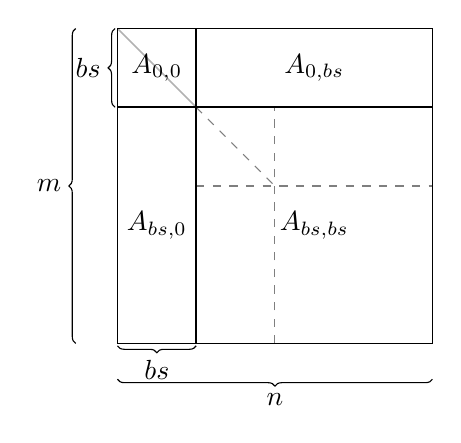
\begin{tikzpicture}
\draw[semithick] (0,0) -- (4,0) -- (4,4) -- (0,4) -- (0,0);

\draw[semithick] (1,0) -- (1,4);
\draw[semithick] (0,3) -- (4,3);
\draw[semithick,opacity=0.3] (0,4) -- (1,3);

\draw[dashed,opacity=0.5] (2,0) -- (2,3);
\draw[dashed,opacity=0.5] (1,2) -- (4,2);
\draw[dashed,opacity=0.5] (1,3) -- (2,2);


\draw (0.5,3.5) node {$A_{0,0}$};
\draw (0.5,1.5) node {$A_{bs,0}$};
\draw (2.5,3.5) node {$A_{0,bs}$};
\draw (2.5,1.5) node {$A_{bs,bs}$};
\draw[decorate, decoration={brace,mirror}, yshift=-.2ex]  (0,0) -- node[below=0.4ex] {$bs$}  (1,0);
\draw[decorate, decoration={brace}, xshift=-.2ex]  (0,3) -- node[left=0.4ex] {$bs$}  (0,4);
\draw[decorate, decoration={brace,mirror}, yshift=-3ex]  (0,0) -- node[below=0.4ex] {$n$}  (4,0);
\draw[decorate, decoration={brace}, xshift=-3.5ex]  (0,0) -- node[left=0.4ex] {$m$}  (0,4);

\end{tikzpicture}
	\caption{Aufteilung der Matrix $A$}
	\label{fig:blockA}
\end{figure}

Die Blockgröße $bs$ wird so gewählt, dass die Geschwindigkeit der ungeblockten QR-Zerlegung für den Block $ \left(\dfrac{A_{0, 0}}{A_{\text{bs}, 0}} \right)$ optimal ist.

Für diesen Block wird die  QR-Zerlegung mit dem ungeblockten Algorithmus (Algorithmus \ref{alg:unblockedqr}) berechnet.
\begin{align}
	\left(\begin{array}{l} 
	A_{0, 0} \\ \hline
	A_{\text{bs}, 0}
	\end{array}\right)
	\leftarrow
	\left(\begin{array}{l} 
	Q_{0, 0}  \backslash R_{0,0} \\ \hline
	Q_{\text{bs}, 0} 
	\end{array}\right)
\end{align}

Im Block $A_{0, 0}$ steht auf und über der Diagonalen $R_{0,0}$. Unterhalb der Diagonalen und im Block $A_{\text{bs}, 0}$ stehen die Householder-Vektoren.

Nun muss man die bei der ungeblocketn QR-Zerlegung verwendeten Housholder-Transformationen auf die restliche Matrix $ \left(\dfrac{A_{0, \text{bs}}}{A_{\text{bs}, \text{bs}}} \right)$ anwenden.

Das Produkt mehrerer Householder-Transformationen kann geschrieben werden als:
\begin{align*}
H_1H_2 \cdot \cdot \cdot H_k = I - VTV^T \qquad \text{mit}\qquad H_i = I - \tau_i v_iv_i^T
\end{align*}  \cite{Joffrain:2006:AHT:1141885.1141886}

Die Anwendung der Householder-Transformationen $I - V*T*V^T$ auf $\left(\frac{A_{\text{bs}, \text{bs}}}{A_{\text{bs}, \text{bs}}} \right)$ erfolgt in 2 Schritten. Zuerst wird  die Matrix $T$ berechnet. Dann wird $I - V*T*V^T$  auf $\left(\frac{A_{\text{bs}, \text{bs}}}{A_{\text{bs}, \text{bs}}} \right)$ angewandt.
%Zuerst wird von der Funktion \glqq larft \grqq{}  die Matrix $T$ berechnet. Dann wird $I - V*T*V^T$ von der Funktion \glqq larfb\grqq{} auf $\left(\dfrac{A_{\text{bs}, \text{bs}}}{A_{\text{bs}, \text{bs}}} \right)$ angewendet.
\begin{align}
	\left(\begin{array}{l} 
	A_{0, \text{bs}} \\ \hline
	A_{bs, \text{bs}}
	\end{array}\right)
	\leftarrow
	H^T \left(\begin{array}{l} 
	A_{0, \text{bs}} \\ \hline
	A_{bs, \text{bs}}
	\end{array}\right)
\end{align}

Der Block $A_{bs, \text{bs}}$ wird erneut aufgeteilt. Das ist in Abbildung \ref{fig:blockA} gestrichelt dargestellt.
Dies wird solange fortgesetzt, bis $A_{bs, \text{bs}}$ gleich der Blockgröße ist.

\subsection{Berechnung der Matrix $T$}
Die Matrix $T$ wird in LAPACK von der Funktion \glqq DLARFT\grqq{} berechnet \cite{LARFT}.

Sie bekommt eine Dreiecksmatrix $V \in \mathbb{R}^{m \times k}$, einen Vektor $\tau \in \mathbb{R}^k$ und eine Matrix $T\in \mathbb{R}^{k\times k}$ übergeben. 

In der Dreiecksmatrix $V$ stehen die Householder-Vektoren,
im Vektor $\tau$ die zu den Householder-Vektoren gehörende $\tau_i$.

Die Funktion berechnet eine obere Dreiecksmatrix $T$ so, dass
\begin{align}
H_1H_2...H_k = I - VTV^T \qquad \text{mit}\qquad H_i = I - \tau_i v_iv_i^T
\label{eq:blkreflectorT}
\end{align}

Warum und wie das Verfahren funktioniert, wird hier beschreiben \cite{Joffrain:2006:AHT:1141885.1141886}.



\begin{algorithm}[H]
\caption{Der Algorithmus berechnet die Matrix $T$ so dass  (\ref{eq:blkreflectorT}) gilt. Die untere Dreiecksmatrix $V$  enthält die Householder-Vektoren. Der Vektor $\tau$ die dazugehörigen $\tau_i = \frac{2}{v_i^Tv_i}$. Hinweise zur Notation: Kleine Buchstaben bezeichnen einen einzelne Matrixeintrag(Beipsiel $v_{i,j}$ ist der Eintrag der i-ten-Zeile und j-ten Spalte der Matrix $V$). Die nach unten gestelletn Indices geben einen Block an der betrachtet werden soll(Beispiel $V_{i:n,j:m}$ bezeichnet einen Block aus der Matrix $V$ der von i-ten bis zur n-ten Zeile und von der j-ten bis zur m-ten Spalte geht).}
\label{alg:clacT}
\begin{algorithmic}[1]
\State Input $V \in \mathbb{R}^{k \times n}$,$\tau \in \mathbb{R}^k$,$T \in \mathbb{R}^{k \times k}$
\For {i = 0,1,2,..., k}
	\If{$\tau_i$ == 0}
		\State $T_{1:i,i}=0$
	\Else
		\State vii$ = v_{i,i}$
		\State $v_{i,i} = 1 $
		%\State T(1:i-1,i) := - $\tau_i$ * V(i:n,1:i-1)' * V(i:n,i)
		\State $T_{0:i,i} = - \tau_i \cdot V_{i:n-i,0:i}^T \cdot V_{i:n-i,i}$ (dgmv)
		\State $ v_{i,i} =$ vii 
		%\State T(1:i-1,i) := T(1:i-1,1:i-1) * T(1:i-1,i)
		\State $T_{0:i,i} = T_{0:i,0:i} \cdot T_{0:i,i}$ (dtrmv)
		\State $t_{i,i} = \tau_i$
	\EndIf
\EndFor
\end{algorithmic}
\end{algorithm}

Der Algorithmus \ref{alg:clacT} überschreibt die Matrix $T$ nach folgendermaßen
\begin{align*}
T =&
\begin{pmatrix}
\tau_1 & -\tau_1 \tau_2 (v_1^T v_2 ) & - \tau_1 \tau_2  \tau_3 (v_1^T v_2 v_2^T v_3) + \tau_1 \tau_3  (v_1^T v_3)\\ 
0 & \tau_2 &  -\tau_2 \tau_3  (v_2^T v_3)\\
0 & 0 & \tau_3
\end{pmatrix}
\end{align*}
Beispiel mit $k=3$

\subsection{Anwenden von $I - VTV^T$}
Die Anwendung der Householder-Transformationen auf eine Matrix $C$ wird in LAPACK von der  Funktion \glqq LARFB\grqq{} implementiert.

Die Funktion bekommt eine untere Dreiecksmatrix $V \in \mathbb{R}^{m \times k}$, eine obere Dreiecksmatrix $T \in \mathbb{R}^{k \times k}$ und eine Matrix $C \in \mathbb{R}^{m \times n }$ übergeben.

In der Dreiecksmatrix $V$ stehen die Householder-Vektoren und $T$ ist die zuvor berechnete Matrix.
Die Matrix $C$ wird upgedatet, indem die Matrix $I - V T V^T $ von rechts auf die Matrix $ C $ angewendet wird. 

Ein weiterer Übergabeparameter gibt an, ob die Matrix  $I - V T V^T $ transponiert werden soll.
Die Funktion berechnet also
\begin{align}
	C \leftarrow H C = C - V T V^T C \quad \text{oder} \quad 	C \leftarrow H^T C = C - V T^T V^T C	\label{eq:larfb}
\end{align}

Der Zweck der Funktion ist es, die Householder-Transformationen die bei der Bereicherung der QR-Zerlegung für einen Block entstanden sind, auf die restliche Matrix anzuwenden.
Die Abbildung \ref{fig:patrA} zeigt, wie die Matrix $A$ für die Funktion partitioniert wird.
\begin{figure} [H]
	\centering
	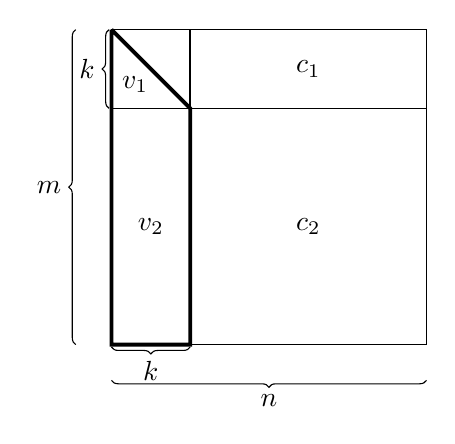
\begin{tikzpicture}
\draw[semithick] (0,0) -- (4,0) -- (4,4)-- (0,4)-- (0,0);


\draw[semithick] (1,0) -- (1,4);
\draw[semithick] (0,3) -- (4,3);
\draw[line width=0.5mm] (0,4) -- (0,0) -- (1,0) -- (1,3) -- (0,4);


\draw[decorate, decoration={brace,mirror}, yshift=-.2ex]  (0,0) -- node[below=0.4ex] {$k$}  (1,0);
\draw[decorate, decoration={brace}, xshift=-.2ex]  (0,3) -- node[left=0.4ex] {$k$}  (0,4);
\draw[decorate, decoration={brace,mirror}, yshift=-3ex]  (0,0) -- node[below=0.4ex] {$n$}  (4,0);
\draw[decorate, decoration={brace}, xshift=-3ex]  (0,0) -- node[left=0.4ex] {$m$}  (0,4);

\draw (0.3,3.3) node {$v_1$};
\draw (0.5,1.5) node {$v_2$};
\draw (2.5,3.5) node {$c_1$};
\draw (2.5,1.5) node {$c_2$};



\end{tikzpicture}
	\caption{Partitionierung vom A für larfb}
	\label{fig:patrA}
\end{figure}
alls $m > k $ werden die Matrizen $V$ und $C$ aufgeteilt in $V=\left(\dfrac{V_1}{V_2}\right)$ und $C=\left(\dfrac{C_1}{C_2}\right)$.
%Sodass $V_1 \in \mathbb{R}^{k \times k}$ und $C \in \mathbb{R}^{k \times n}$
Dabei wird $V$ genau so geteilt, dass $V_1 \in \mathbb{R}^{k\times k}$ der quadratisch Dreiecksteil der Matrix ist und $V_2 \in \mathbb{R}^{m-k\times k}$ der Rest der Matrix. Die Matrix $C$ wird in $C_1 \in \mathbb{R}^{k \times n}$ und $C_2 \in \mathbb{R}^{m-k \times n}$  aufgeteilt. Die Aufteilung ist so gewählt, dass das Matrix-Matrix-Produkt $V_1 \cdot C_1$ und $V_2 \cdot C_2$ möglich ist.\\
Diese Aufteilung ist notwendig, da die BLAS-Funktion trmm (matrix-matrix product where one input matrix is triangular) nur für quadratische Dreiecksmatrizen implementiert ist.

Im Fall $ m = k $ ist die Aufteilung nicht notwendig, da $ V $ quadratisch ist.

(\ref{eq:larfb}) kann mit der Umformung
\begin{align*}
	C &\leftarrow  C - V T V^T C \\
	C &\leftarrow C - (V T V^T C)^{TT} 	\\
	C &\leftarrow  C - (C^T  V  T^T  V^T)^T
\end{align*}
mit BLAS-Routinen wie in Algorithmus \ref{alg:applyblockref} berechnet werden.

\begin{algorithm}[H]
	\caption{$I - V T V^T$ auf C anwenden.\\
			 Die Matrix $W$ ist ein Workspace}
	\label{alg:applyblockref}
	\begin{algorithmic}[1]
		\State Input: $V \in \mathbb{R}^{m \times k}$, $T \in \mathbb{R}^{k \times k}$, $C \in \mathbb{R}^{m \times n}$
		\State 	$W \leftarrow C_1^T$ (copy)
		\State	$W \leftarrow W * V_1 $ (trmm)
		\If {m > k}
			\State $W \leftarrow W + C_2^T*V_2$ (gemm)
		\EndIf
		\State 	$ W \leftarrow W * T^T \quad \text{or}\quad  W * T$ (trmm)
		\If {m > k}
			\State $C_2 \leftarrow C_2 - V_2 * W^T$ (gemm)
		\EndIf
		\State 	$ W \leftarrow W * V_1^T $ (trmm)
		\State 	$ C_1 \leftarrow C_1 - W^T $
	\end{algorithmic}
\end{algorithm}


%\subsection{Iterativer Algorithmus}
%\begin{algorithm}[H]
%	\caption{Iterativer Algorithmus}
%	\label{alg::italg}
%	\begin{algorithmic}
%		\For {i = 0 : n}
%			\State QR = A;
%			\If {i + ib > n}
%				\State Calc T: $H=I-VTV^T$
%				\State Apply H: $A=H^TA$
%			\EndIf
%		\EndFor
%	\end{algorithmic}
%\end{algorithm}
